\documentclass[tikz, border=10pt]{standalone}
\usetikzlibrary{decorations.pathreplacing, positioning}

\begin{document}
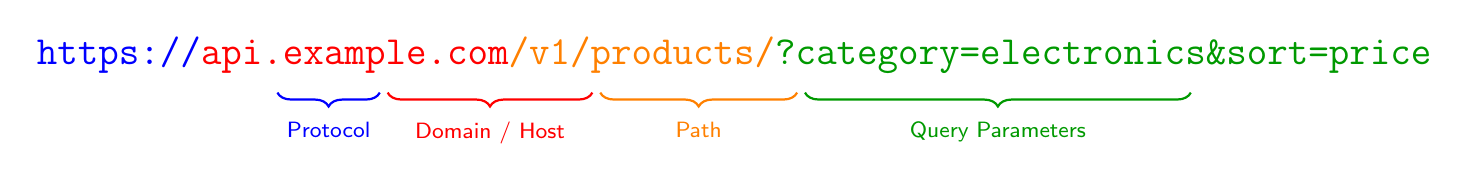
\begin{tikzpicture}[font=\sffamily\footnotesize]

\node (url) {\Large \texttt{\textbf{\textcolor{blue}{https://}}\textcolor{red}{api.example.com}\textcolor{orange}{/v1/products/}\textcolor{green!60!black}{?category=electronics\&sort=price}}};

\draw [thick, decorate, decoration={brace, amplitude=5pt, mirror, raise=5pt}, blue] 
    (-5.8,-0.3) -- (-4.5,-0.3) node [midway, below=12pt] {Protocol};

\draw [thick, decorate, decoration={brace, amplitude=5pt, mirror, raise=5pt}, red] 
    (-4.4,-0.3) -- (-1.8,-0.3) node [midway, below=12pt] {Domain / Host};

\draw [thick, decorate, decoration={brace, amplitude=5pt, mirror, raise=5pt}, orange] 
    (-1.7,-0.3) -- (0.8,-0.3) node [midway, below=12pt] {Path};

\draw [thick, decorate, decoration={brace, amplitude=5pt, mirror, raise=5pt}, green!60!black] 
    (0.9,-0.3) -- (5.8,-0.3) node [midway, below=12pt] {Query Parameters};

\end{tikzpicture}
\end{document}

